\section{Methodology}
\label{sec:methodology}
Figure~\ref{fig:rigor-method} summarizes the pipeline. Each stage writes inspectable artifacts, allowing an end-output error to be traced to geometry, detection, relation assignment, or structured export.

\begin{figure*}[t]
  \centering
  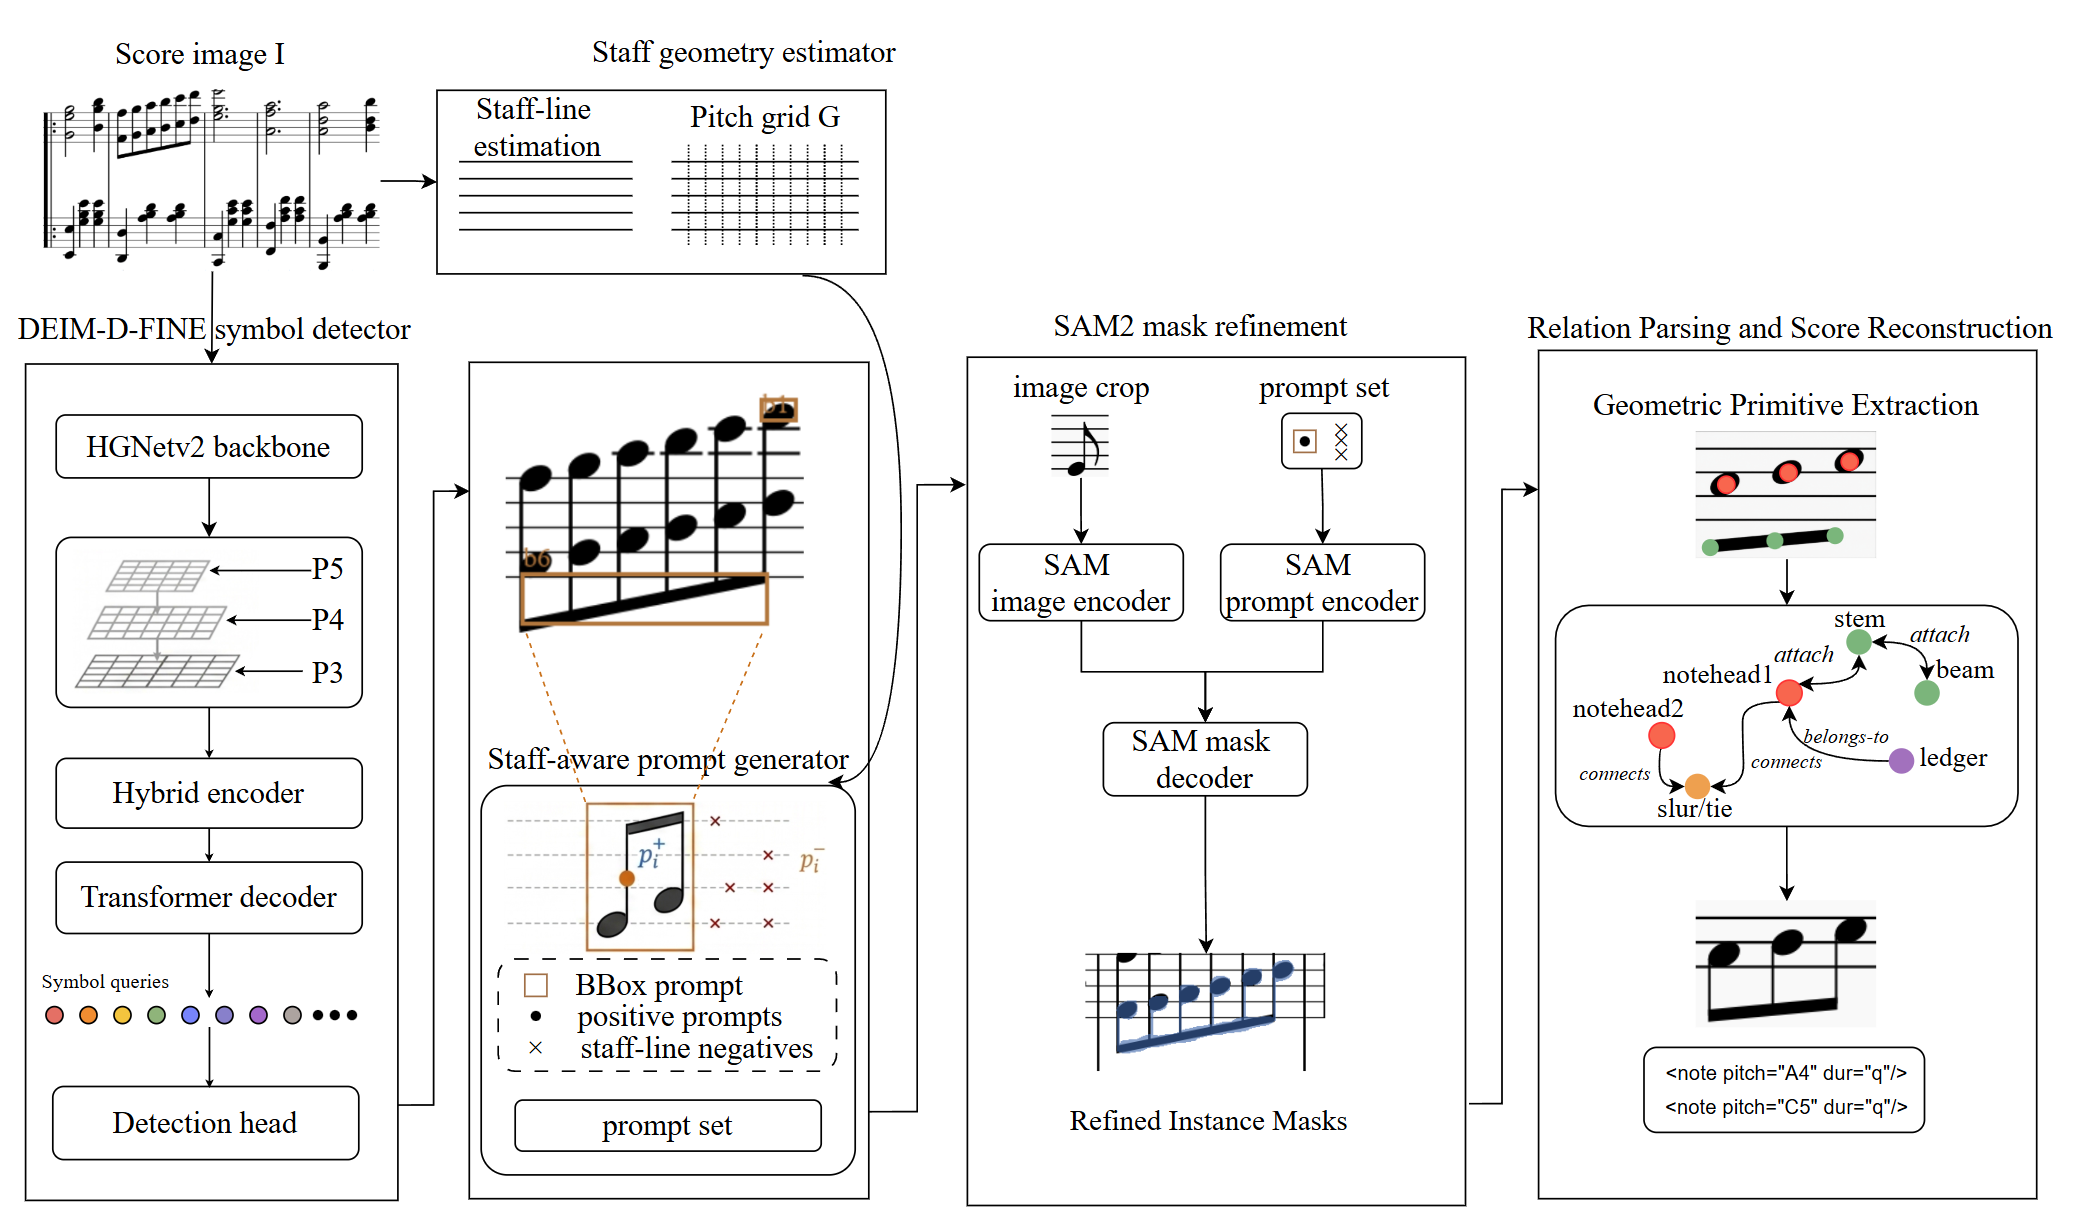
\includegraphics[width=\textwidth]{figure/rigor_omr_method.png}
  \caption{Overview of RIGOR-OMR. A staff-geometry estimator defines a normalized pitch grid; DEIM-D-FINE detects notation symbols; staff-aware prompts guide optional SAM2 mask refinement; and typed geometric relations support pitch--duration event assembly and structured score reconstruction.}
  \label{fig:rigor-method}
\end{figure*}

\subsection{Staff Geometry Estimation}
Given a score image $I$, horizontal projections and connected components identify five-line staff groups. For staff $k$, the line coordinates $\{\ell_{k,j}\}_{j=1}^{5}$ define the robust spacing
\begin{equation}
 s_k=\operatorname{median}_{j=1}^{4}(\ell_{k,j+1}-\ell_{k,j}).
\end{equation}
The lines and inter-line half spaces form a discrete pitch grid $G_k$. We express box sizes, attachment distances, and prompt offsets in units of $s_k$, so the downstream rules remain comparable across resolution and engraving scale. The geometry stage outputs staff regions, line coordinates, normalized symbol coordinates, and candidate pitch-grid positions.

\subsection{Staff-Aware Symbol Detection}
The score image is processed by a 58-class DEIM-D-FINE detector. Its HGNetv2 backbone and hybrid encoder produce multiscale features, while symbol queries predict class-labeled boxes \cite{huang2025deim,peng2025dfine}. Depending on page shape, inference uses either the resized full page or overlapping page-coordinate tiles; predictions are merged by class-aware non-maximum suppression. Each detection $d_i=(b_i,c_i,q_i)$ contains a box $b_i$, symbol class $c_i$, and confidence $q_i$; overlap with the estimated staff regions assigns it to a staff and maps its center to normalized grid coordinates. The frozen runs use a separate four-way clef ROI classifier where enabled; it cannot relabel non-clef symbols.

\subsection{Staff-Aware Prompt Generation and Mask Refinement}
For each detection $d_i$, the frozen main run passes its unexpanded box $b_i$ to SAM2.1 Hiera-Tiny as a box-only prompt \cite{ravi2025sam2}. Positive points and staff-line negative points are reserved for prompt-strategy ablations and are not part of the reported default. SAM2 is frozen and acts as an optional boundary refiner rather than a notation classifier; this distinction matches the factorial ablation in Section~\ref{sec:factorial}, where masks improve inspectability but not the final Event-F1.

\subsection{Geometric Primitive Extraction and Relation Parsing}
Each refined instance mask is converted into an appropriate primitive: polygons for area-like noteheads and accidentals, and pruned skeletons or endpoints for stems, beams, ledger lines, barlines, and slurs. Every primitive becomes a typed node $v\in V$ with class, staff index, box, mask evidence, and staff-normalized coordinates. RIGOR-OMR then constructs $G=(V,E)$ using class-compatible geometric candidates. Notehead--stem edges require horizontal compatibility and a bounded endpoint distance; stem--beam edges require proximity between a stem endpoint and beam support. Ledger--notehead, accidental--notehead, and slur/tie endpoint candidates use analogous type-specific constraints. Conflict pruning retains a consistent set of attachments before event assembly.

\subsection{Global Structure Decoder}
The upgraded reconstruction backend converts connected primitives into musical events and then decodes a canonical score order; it is a deterministic backend upgrade rather than an additional learned model. The clef-conditioned grid $G_k$ determines pitch, while stem, beam, flag, and dot evidence determines duration, and relation edges bind these attributes to the same event. The decoder groups staves into piano systems, obtains shared measure partitions from supported barlines, clusters staff-normalized horizontal coordinates into onset hypotheses, groups compatible simultaneous notes into chords, and serializes in system--measure--onset--staff order with deterministic pitch and geometry tie breaking. It exports both an auditable event representation and MusicXML or a dataset-compatible proxy sequence. Because decoding is deterministic once $V$ and $E$ are fixed, relation families can be removed and the score rebuilt without retraining or rerunning the detector, enabling the controlled edge ablations in Section~\ref{sec:relations}.

\FloatBarrier
